\documentclass[output=paper,draftmode,colorlinks,citecolor=brown]{langscibook}
\ChapterDOI{10.5281/zenodo.15006593}
\author{Kimberley Baxter\affiliation{New York University}}

\title{Extracting “non-standard” data from the Twitter API}

\abstract{The present paper examines methodology in the use of Twitter in the corpus-based analysis of African American English (AAE) syntax. I discuss the extraction and geospatial mapping of indices of use of the perfective marker \textit{done} (hereafter  \textit{perfective done}), which, alongside a simple past form, indicates that the action described in the past form has been completed. Widespread use of AAE on archived social media posts creates a living database of timed, dated, and geotagged utterances from which corpora may be built. The Academic Twitter API (ACTW) allows access to their full database of tweets, which is a much larger and more accessible dataset than its large social media contemporaries. I discuss two methods of extracting perfective \textit{done} from the ACTW: a \textit{front-end} approach which aims to isolate uses of perfective \textit{done} by eliminating non-perfective uses of \textit{done} from the search prior to running the query, and a \textit{back-end} approach which first extracts a set of all uses of \textit{done} from 2012--2015 and aims to isolate uses of perfective \textit{done} afterwards. I discuss the results of this method, as well as the implications therein and directions for future research. I conclude that while both methods are effective at extracting perfective \textit{done} from the ACTW, the \textit{back-end} approach is better suited to geospatial mapping.}
\IfFileExists{../localcommands.tex}{
  \addbibresource{../localbibliography.bib}
  \usepackage{tabularx,multicol}
%\usepackage{multirow}
\usepackage{subcaption}
\usepackage{url}
\urlstyle{same}

\usepackage{datetime}
\usepackage{enumitem}
\usepackage{langsci-optional}
\usepackage{langsci-lgr}
\usepackage{langsci-branding}

\usepackage{longtable}
\usepackage{xltabular}
\usepackage[linguistics, edges]{forest}
\usepackage{pgfplots}
\pgfplotsset{compat=1.18}
\usetikzlibrary{patterns, tikzmark}
\usepackage{pgfplotstable}
\usepgfplotslibrary{colorbrewer}
\usepackage{listings}
\lstset{basicstyle=\ttfamily,keywordstyle=\normalfont,language=,breaklines=true}

\usepackage{siunitx}
\sisetup{group-digits=none, detect-all=true}

\usepackage{langsci-gb4e}

  \makeatletter
\let\thetitle\@title
\let\theauthor\@author
\makeatother

% Use this Chinese font shipped with TeX Live instead of Source Han, because
% it is more portable/leightweight. Install the "fandol" package from CTAN to
% automatically get this font.
\newfontfamily{\ChineseFandolSong}{FandolSong-Regular.otf}

  %% hyphenation points for line breaks
%% Normally, automatic hyphenation in LaTeX is very good
%% If a word is mis-hyphenated, add it to this file
%%
%% add information to TeX file before \begin{document} with:
%% %% hyphenation points for line breaks
%% Normally, automatic hyphenation in LaTeX is very good
%% If a word is mis-hyphenated, add it to this file
%%
%% add information to TeX file before \begin{document} with:
%% %% hyphenation points for line breaks
%% Normally, automatic hyphenation in LaTeX is very good
%% If a word is mis-hyphenated, add it to this file
%%
%% add information to TeX file before \begin{document} with:
%% \include{localhyphenation}
\hyphenation{
    a-na-ly-sis
    ap-proach-es
    ar-che-o-log-i-cal
    Ar-khan-gelsk
    be-schrei-ben
    Buch-holtz
    Che-lya-binsk
    con-so-nant
    dia-lect
    dia-lect-ology
    Di-a-lekt-for-schung
    Dia-lekt-for-schung
    East-pha-lian
    För-der-ung
    Ge-mein-schaft-lich-keits-ent-wür-fe
    his-tor-i-cal
    Hok-kai-do
    ja-pa-nese
    Ja-pa-nese
    Ka-go-shi-ma
    Ka-li-nin-grad
    Knja-zev
    Ma-kro-be-reich
    Ma-lay-sia
    mor-pho-log-i-cal
    Mos-cow
    Nef-te-yu-gansk
    non-mobile
    nu-cle-ar
    ös-ter-rei-chi-sche
    par-a-digm
    per-zep-ti-ons-lin-gu-is-ti-sche
    plu-ri-zen-tri-schen
    quick-ly
    Reich
    Sax-on
    Schrö-der
    sear-ching
    ste-reo-type
    strength-en-ing
    strong-est
    Stutt-gart
    su-pra-seg-men-tal
    teach-er
    to-po-gra-phy
    To-ron-to
    tra-di-tion-al
    ul-ti-mate-ly
    Um-gangs-spra-che
    Volks-kun-de
    vor-zu-stel-len
    wheth-er
    Wie-sing-er
    with-in
    Wort-at-las
}

\hyphenation{
    a-na-ly-sis
    ap-proach-es
    ar-che-o-log-i-cal
    Ar-khan-gelsk
    be-schrei-ben
    Buch-holtz
    Che-lya-binsk
    con-so-nant
    dia-lect
    dia-lect-ology
    Di-a-lekt-for-schung
    Dia-lekt-for-schung
    East-pha-lian
    För-der-ung
    Ge-mein-schaft-lich-keits-ent-wür-fe
    his-tor-i-cal
    Hok-kai-do
    ja-pa-nese
    Ja-pa-nese
    Ka-go-shi-ma
    Ka-li-nin-grad
    Knja-zev
    Ma-kro-be-reich
    Ma-lay-sia
    mor-pho-log-i-cal
    Mos-cow
    Nef-te-yu-gansk
    non-mobile
    nu-cle-ar
    ös-ter-rei-chi-sche
    par-a-digm
    per-zep-ti-ons-lin-gu-is-ti-sche
    plu-ri-zen-tri-schen
    quick-ly
    Reich
    Sax-on
    Schrö-der
    sear-ching
    ste-reo-type
    strength-en-ing
    strong-est
    Stutt-gart
    su-pra-seg-men-tal
    teach-er
    to-po-gra-phy
    To-ron-to
    tra-di-tion-al
    ul-ti-mate-ly
    Um-gangs-spra-che
    Volks-kun-de
    vor-zu-stel-len
    wheth-er
    Wie-sing-er
    with-in
    Wort-at-las
}

\hyphenation{
    a-na-ly-sis
    ap-proach-es
    ar-che-o-log-i-cal
    Ar-khan-gelsk
    be-schrei-ben
    Buch-holtz
    Che-lya-binsk
    con-so-nant
    dia-lect
    dia-lect-ology
    Di-a-lekt-for-schung
    Dia-lekt-for-schung
    East-pha-lian
    För-der-ung
    Ge-mein-schaft-lich-keits-ent-wür-fe
    his-tor-i-cal
    Hok-kai-do
    ja-pa-nese
    Ja-pa-nese
    Ka-go-shi-ma
    Ka-li-nin-grad
    Knja-zev
    Ma-kro-be-reich
    Ma-lay-sia
    mor-pho-log-i-cal
    Mos-cow
    Nef-te-yu-gansk
    non-mobile
    nu-cle-ar
    ös-ter-rei-chi-sche
    par-a-digm
    per-zep-ti-ons-lin-gu-is-ti-sche
    plu-ri-zen-tri-schen
    quick-ly
    Reich
    Sax-on
    Schrö-der
    sear-ching
    ste-reo-type
    strength-en-ing
    strong-est
    Stutt-gart
    su-pra-seg-men-tal
    teach-er
    to-po-gra-phy
    To-ron-to
    tra-di-tion-al
    ul-ti-mate-ly
    Um-gangs-spra-che
    Volks-kun-de
    vor-zu-stel-len
    wheth-er
    Wie-sing-er
    with-in
    Wort-at-las
}

  \togglepaper[1]%%chapternumber
}{}

\begin{document}
\maketitle
\label{chap:baxter}
\shorttitlerunninghead{Extracting “non-standard” data from the Twitter API}%%use this for an abridged title in the page headers
% ATTENTION: Diacritics on the following phonetic characters might have been lost during conversion: {'ə'}
\graphicspath{{figures/baxter}}



\section{Introduction}
\label{sec:baxter:1}
\subsection{General remarks} %1.1 /
\label{sec:baxter:1.1}
Despite longstanding myths of African American English (AAE) as a linguistic monolith \citep{Wolfram2007}, numerous sociolinguistic studies indicate that AAE shows regional variation in both phonology and lexicon (see \citealt{Wolfram2007, Lanehart2015}, etc. for phonology; \citealt{Jones2015, Grieve2016}, etc. for lexicon). Far fewer studies focus on syntactic variation in AAE across regions, and of those that do, many are restricted to a certain geographic area (e.g. \citealt{Terry2010, Moody2011}), with \citet{chapters/01-baxter, chapters/02-baxterEtAl}, and \citet{MasisEtAl2022} constituting notable exceptions. This study aims to fill this gap by using geotagged Twitter data to investigate syntactic variation in AAE across the contiguous United States.

The goals of this study are to:

\begin{itemize}
\item[a)] Present a method for the targeted search of AAE parts of speech which maximizes the number of desired features while minimizing the number of false positive features, which are orthographically identical to the desired feature, yet still syntactically different;

\item[b)] Calculate indices which reflect the rate of feature use by geographical region;

\item[c)] Correlate these indices with demographic data to discover whether indices of feature use vary across locations with a high density of Black/African American people.
\end{itemize}


By doing so, this paper seeks to address the myth of supraregionality in AAE \citep{Wolfram2007}, which suggests nationwide grammatical universality in urban centers (see \sectref{sec:baxter:1.2}).

This paper focuses on the methodology used to plot the geographic distribution of one such feature canonical to AAE: perfective \textit{done} (\cite{Rickford1999, Green2002, Green2010}). I describe two approaches to the collection of perfective \textit{done} tokens from the Academic Twitter API (ACTW): a \textit{front-end} approach, through which grammatical restrictions are applied prior to extracting tweets, resulting in a dataset comprised mostly of tweets using perfective \textit{done}, and a \textit{back-end} approach, through which grammatical restrictions are applied after extracting tweets, resulting in a dataset comprised of all uses of \textit{done}, from which a subset of perfective \textit{done} may be extracted.

\subsection{African American (Vernacular) English} %1.2
\label{sec:baxter:1.2}
This paper uses \textit{African American English} (AAE) to describe the language previously known as \textit{African American Vernacular English} (AAVE), \textit{Black Vernacular English} (BEV), etc. In doing so, I aim to distance myself from the “vernacularization” of AAE introduced by previous research which focused mainly on male street youth in the inner city (e.g. \cite{Labov1972}). AAE is one of many African American languages which fall under the umbrella of AAL, including, but not limited to, Gullah Geechie, Black American Sign Language, Louisiana Creole, and many more. AAE is a sociolect spoken mostly by Black Americans and people who live in community with Black Americans. In discussing AAE, it is also important to consider race and ethnicity in the United States and how that informs not only what AAE is, but who speaks it, and how African American and other Black people in the US are categorized demographically (see \citet{Blake2014} and \citet{King2020}, both of which speak to issues of the racialization and categorization of AAE).

The US Census does not account for differences in ethnicity among Black people in the United States -- instead, all Black-identifying people are encompassed within the same singular category, \textit{Black/African American}. This category only seeks specification regarding whether one is “Black/African American alone” or “in combination” with other races/ethnicities. This is an issue which affects all studies of AAE which seek to utilize the US Census as a touchstone for demographic metadata, including the proposed dissertation. I use \textit{Black/African American} (henceforth: BAA) in discussions regarding the racial and ethnic identity of Black people in this paper.

\subsection{Why investigate variation in AAE?}  %1.3 /
\label{sec:baxter:1.3}
While research on the systematicity of AAE sparked a groundbreaking shift in Sociolinguistics as a whole, researchers also inadvertently established a series of myths about AAE and its uniformity \citep{Wolfram2007}:


\ea The Supraregional Myth: primary structural features setting apart the vernacular speech of African Americans from their European American cohorts were shared by African American Communities regardless of regional context.
\z

\ea The Language Change Myth: a uniform path of change for African American English, based on the uniformity of AAE
\z

\ea The Social Stratification Myth: the prevailing assumption that African American English is most commonly used by working-class speakers, especially those who have had little to no contact with other varieties of English.
\citep[295--306]{Wolfram2007}
\z

\newpage
These myths persist among the definitions of AAE in previous literature:

\begin{quote}

[AAE is] the uniform grammar used by African Americans who have minimal contact with other [varieties] in contexts where only speakers of that vernacular are present. (\citealt{Baugh1983}, as cited by \citealt[6]{Labov1998})\\
Due to sociopsychological barriers between Blacks and Whites, AAE is a marker of identity. This causes uniformity among Blacks from all over the US. (\citealt{Rickford1999}, as cited by \citealt[20]{Johnson2008})
\end{quote}

The impression of AAE as a “uniform” sociolect is widespread in previous literature on AAE. While these definitions were published decades ago, this myth of uniformity across regions, also known as \textit{supraregionality}, still persists in more recent literature. \citet{Wolfram2007} goes into great detail about all three of these myths, but the most salient of these for the purpose of this paper is the Supraregional Myth. While the papers cited in \citet{Wolfram2007} were from decades earlier, this myth is still very much present in relatively recent literature, as seen below:

\begin{quote}
\sloppy\relax
[AAE] is, in contrast to other North American [varieties], not geographically restricted. Although variation in AAE does exist, AAE in urban settings has been established as a uniform system with suprasegmental norms… \citep[10]{JørgensenHovySøgaard2015}
\end{quote}

The use of Twitter as a source of data allows researchers to collect far more data than would be possible via traditional methods such as surveys and sociolinguistic interviews. Twitter’s Academic Developer License (ADL) allows access to Twitter’s entire archive of tweets, from which a maximum of 10,000,000 tweets may be mined per ADL, per month. Because the archived tweets were produced voluntarily by Twitter users, this method may also circumvent the Observer's Paradox \citep{Labov1972} and similar issues which often arise during the process of face-to-face data collection. The use of Twitter data also presents a boon for the collection of parts of speech which are more difficult to elicit via interviews because of the presence of linguistic alternatives, through which similar meanings and ideas may be conveyed. For example, where my previous attempts at eliciting perfective \textit{done} from interviews yielded very few results, Twitter allows me to pinpoint parts of speech associated with AAE (\citealt{Green2002, Rickford1999}) specifically. This data can then be mapped geospatially via the metadata included with each tweet and provide insight on the geographical distribution of perfective \textit{done}.

\section{Analyzing language variation in social media}
\label{sec:baxter:2}
There are well-documented challenges analyzing non-standard varieties of English commonly used in social media \citep{plank-etal-2016-multilingual}, and AAE is no different. These challenges fit into two broad categories: grammatical challenges, and demographic challenges. I discuss each of these challenges below.

\subsection{Grammatical challenges}
\label{sec:baxter:2.1}
Standard methods of extracting data from Twitter’s APIs often lack the specifications necessary to isolate parts of speech exclusive to AAE, and differentiate them from similar lexical items in Mainstream American English (MAE) \citep{JørgensenHovySøgaard2015}. This is in part because AAE has a robust verbal system which allows its verbal lexicon to be used as aspect and mood/modality markers in addition to their use as tense markers, as seen below in examples \REF{ex:baxter:4}, \REF{ex:baxter:5}, and \REF{ex:baxter:6}. \REF{ex:baxter:4} is an example of perfective \textit{done}), indicating that the action of going to the store has been completed. Example \REF{ex:baxter:5} shows perfective \textit{done} being used in conjunction with the simple past form of the verb \textit{do}. Example \REF{ex:baxter:6} shows perfective \textit{done} being used in conjunction with \textit{do} in its participle form.

\ea \label{ex:baxter:4}
He done   went   to the store already. \\
He \textsc{perf}   went   to the store already. \\
\glt ‘He has gone to the store already.’
\ex \label{ex:baxter:5}
He done   did     his work. \\
He \textsc{perf}   did   his work.\\
\glt ‘He has done his work.’
\ex \label{ex:baxter:6}
Now look what you done done. \\
Now look what you \textsc{perf} \textsc{part}. \\
\glt ‘Now look what you’ve done.’
\z

All three of these examples are grammatically correct in AAE, yet the perfect and participle forms of \textit{done} in \REF{ex:baxter:6} are orthographically identical. For the purpose of this paper, an alternate form of \textit{done} which is grammatically different, yet orthographically identical to perfective \textit{done} is called a \textit{false positive} (FP). Conducting a simple search for the word \textit{done} in the ACTW results in a high number of FPs and data which renders the manual elimination of FPs unfeasible due to the sheer size of the dataset, which numbers in the millions of tweets (see \sectref{sec:baxter:4}).

This paper ultimately aims to produce an alternative method which allows the user to eliminate the aforementioned FPs by coding the grammatical constraints of perfective \textit{done}, which would otherwise be inaccessible due to the lack of highly accurate part of speech taggers designed for this task. While the focus of this research is on Twitter, I raise further questions about language variation in AAE in \sectref{sec:baxter:7}.

\subsection{Demographic challenges}
\label{sec:baxter:2.2}

Tracking variation in a sociolect such as AAE is difficult on social media sites which grant anonymity to its millions of users. In the case of Twitter, with the exception of verified profiles (indicated with a blue check), confirmation of one’s race, ethnicity, gender, or other facets of one’s identity are completely optional. As a result, a reliable mass verification of users’ demographic data is not currently feasible. 


Multiple surveys have been conducted in an effort to tease apart the demographics of Twitter, with varying results. This study refers to the 2018 Pew Research Study “Sizing Up Twitter” to describe the broad demographics therein. “Sizing Up Twitter” is a representative survey of 2791 adult Twitter users surveyed via Ipsos KnowledgePanel, a probability-based online panel of US adults. The survey found that at the time of the study, approximately 80\% of all tweets were made by 10\% of Twitter users. Twitter users tended to be younger, and more likely to be Democrat or otherwise left-leaning, more likely to be women, and more likely to tweet about politics. Eleven percent of Twitter users identify as Black* (not including Black people who also identify as Hispanic). Of these, approximately 30\% are college graduates, 40\% have some college education, and 30\% have a high school diploma or have not completed their high school education. The survey does not include statistics on political affiliation, age, or use \textit{by race}. 

However, the study does present a representative Twitter demographic which shows a percentage of Black tweeters which is comparable to the general population of the United States in the same year (approximately 13\% of the total population of the United States; \citealt{Bureau2018}). The US Census Bureau recorded 22.5\% of the Black population in the United States 25 years and older as having a bachelor’s degree in 2015 \citep{RyanBauman2015}. While there are some gaps between the “Sizing Up Twitter” dataset and the US Census Bureau dataset, the lower percentage of college graduates in the US Census Bureau dataset appears to support the finding that Black Twitter users are also more likely to be college educated than the general population.

With the recent the recent sale and transformation of Twitter (now X) under the ownership of Elon Musk, the demographics therein, especially along racial and political lines, may now be very different. In a Washington Post article entitled “Fleeing Elon Musk's X, the quest to re-create ‘Black Twitter’”, \citet{Dwoskin2023} describes a political shift in Twitter's formerly left-leaning environment:


\begin{quote}
Hate speech has surged on the platform. Researchers with the Network Contagion Research Institute (NCRI), a group that analyzes hundreds of millions of messages across social media, discovered an account that included a Nazi swastika in its profile picture tweeting antisemitic memes. Use of the n-word soared by nearly 500 percent, and the slur popped up in the handle of an account authorized by Musk’s subscription service, Twitter Blue. And thus the exodus of Black users began.
\citep{Dwoskin2023}
\end{quote}


The data used in both this paper and \citet{chapters/02-baxterEtAl} was produced by its users and collected from the ACTW prior to many of these changes, and are reflective of the Twitter captured in \citet{WojcikHughes2019}. In addition, the talk from which this paper is derived was given before Twitter became X. For the sake of consistency, this paper uses Twitter to refer to the social media platform now known as X. In addition, there does not appear to be a new term for posts made on the platform; as a result, this paper also maintains \textit{tweet}(\textit{s}) as the label for posts made therein.

Since this talk was given, the ACTW has been discontinued, or at the very least paused, preventing the collection of further data from this source. However, it is my belief that these methods will still prove useful to researchers who wish to extract “non-standard” data from similar social media APIs, including X’s new Enterprise API product.

\subsection{Linguistic grouping approach}
\label{sec:baxter:2.3}

Because of the relative anonymity of Twitter profiles, this study uses a “linguistic grouping” approach \citep{HorvathSankoff1987}, through which linguistic features of AAE are collected and analyzed \textit{before} the categorization and analysis of sociological factors such as race and ethnicity. This method is preferred to the traditional “sociological grouping” approach used in most traditional sociolinguistic studies which, because of the aforementioned anonymity of Twitter profiles, makes it difficult to verify the ethnicities of the users behind each account.

\begin{quote}
The terms social and linguistic grouping do not mean that sociological consideration predominate in one approach and linguistic concerns in the other, but only refer to the temporal order in which they enter into the statistical analysis. \citep[180]{HorvathSankoff1987}
\end{quote}

The present study starts by choosing a linguistic variable, in this case perfective \textit{done}, and calculating indices of use, mapped across the contiguous United States via the geolocation metadata attached to each tweet. These indices are then compared to indices of BAA population in US Census tracts across the contiguous United States. By doing so, I aim to provide a broad yet comprehensive view of perfective \textit{done} usage rates in high-density BAA communities.



I plan to conduct future research (see \sectref{sec:baxter:7}) to properly investigate language differences among first- and second-generation Black immigrants’ AAE and the AAE spoken by Black people who are ethnically African American. However, this is beyond the scope of this paper, as well as the limits of what Twitter data or US Census data can currently offer.


\section{Perfective \textit{done}}
\label{sec:baxter:3}

Similarly to \citet{BlodgettGreenO’Connor2016}, \citet{Stevenson2016}, and \citet{Willis2020}, the present study aims to examine syntactic variables in AAE. This should not be confused with studies on the spread and use of lexical items in AAE such as \textit{fleek} \citep{Grieve2016}, \textit{eem} \citep{Jones2015}, or others. This distinction is very important because AAE has a robust verbal system which allows the use of verbal items as tense, mood\slash modality, and aspect markers. It is not enough to simply search the ACTW for all uses of \textit{done}, \textit{be}, \textit{BIN} (spelled \textit{been} by AAE speakers), or any other part of AAE speech. One must be familiar with the syntactic properties of these items and devise alternate strategies to separate them from their verbal, adjectival, or other counterparts when extracting data from the ACTW. It is with that in mind that I discuss perfective \textit{done.}


\citet{Green2002} describes perfective \textit{done} below. Numbers have been changed for continuity within the present paper:


\ea
\ea
I told him you dən changed. (Bm, 30’s)\\
\glt ‘I told him that you have changed.’\\
A:\quad You through with Michael Jordan I bought you? \\
(Literally: Have you finished reading the magazine that I bought you with Michael Jordan on the cover?)\\
B:\quad I dən already finished that. (Bm, 9)\\
\glt ‘I have already finished that.’

\ex I dən done all you told me to do. I dən visited the sick. (Bm, 60s, 70s) \\
‘I have done all you told me to do. I have visited the sick.’\\
\ex
A:\quad Push your seat.\\
B:\quad I dən pushed it.\\
\glt ‘I have (already) pushed it.’ \\
A:\quad Push it again. (elderly Bfs on Amtrak)\\
\citep[60]{Green2002}
\z
\z

\ea \label{ex:baxter:8}
\ea My homework is \textit{done}.
\ex Have you \textit{done} your taxes?
\z
\z

Perfective \textit{done} is distinct from \textit{done} in its verbal or adjectival form as seen above in example \REF{ex:baxter:8} and is most often compared to the MAE perfect markers \textit{have}, \textit{has}, and \textit{had}.

Perfective \textit{done} typically occurs with both stative and eventive verbs, as well as time adverbs and negation \citep{Martin2018}. The present study uses the descriptor \textit{perfective} rather than \textit{completive} because \textit{perfective} is inclusive of uses of \textit{done} which indicate that an action, event, or status has been completed, as well as uses of \textit{done} which indicate that an action, event, or status is still ongoing.

Due to its ability to describe completed actions, events, or statuses, perfective \textit{done} often appears with eventive verbs, which have a natural endpoint. However, in certain contexts, perfective \textit{done} can occur with stative verbs, which do not have natural endpoints. For example, the following sentence includes perfective \textit{done} with the stative verb \textit{know}:

\ea%9
    \label{ex:baxter:9}
    \gll Long as I done known you (you’ve been chasing after women) \\
         \textsc{tmp-}long   as I \textsc{perf} known you (you’ve been chasing after women) \\
    \glt ‘For as long as I have known you (you’ve been chasing after women).’ (\citet{Wilson1986}, cited in \citet{Martin2018})
\z


\citet{Terry2010} argues that \textit{done} is perfective because it fits the “four perfect constructions” as outlined in \citet{Comrie1976}:

\ea%10
\label{ex:baxter:10}
Perfect of persistent situation: this perfect behaves similarly to stative BIN, in that it indicates that an event began in the past, and is still occurring.\\

“Mary \textit{done} lived in Chapel Hill for 6 years.”\\

The above example indicates that Mary has been living in Chapel Hill since the distant past, and still does.
\z

\ea%11
    \label{ex:baxter:11}
    Experiential perfect: indicates that a situation took place or held at some time in the past.\\

“They \textit{done} took my car.”\\
\z

\ea%12
    \label{ex:baxter:12}
  Perfect of result: the present state is referred to as being the result of the past. \\

“And now you \textit{done} messed everything up.”\\
\z

\ea%13
\label{ex:baxter:13}
 Perfect of recent past: temporal closeness to the present is the focus, rather than the completion.\\
“John \textit{done} just got here.”\\
\z

\citet{Terry2010} notes that perfective \textit{done} expresses the “continuing relevance of a previous situation” \citep[56]{Comrie1976} and, as a result, appears to fit the criteria of a perfect marker.

However, it is important to note that while \citet{Terry2010} makes a convincing argument as to why \textit{done} should be a perfective, the use of the “four perfect” structure in \citet{Comrie1976} does not adequately describe perfective \textit{done} in AAE. Certain uses of perfective \textit{done} do not fit neatly into these categories and can even occupy multiple categories at once. For example, when asking informally about the categorization of the utterance listed in example \REF{ex:baxter:9}, \textit{Mary done lived in Chapel Hill for 6 years}, several AAE speakers agreed with the judgment that it meant \textit{Mary} still lived there while others disagreed, stating that \textit{Mary} lived there already and now lived somewhere else.  This difference in interpretation may be the result of several factors including context taken from voice intonation, context from previous portions of the conversation, or in some cases a lack of context as a result of the utterance being written via text or survey.

In addition, while perfective \textit{done} can be compared to use of the perfect in MAE (\textit{have}, \textit{has}, \textit{had}), it is not grammatically \textit{identical} to the perfect in MAE \citep{Martin2018}.

Perfective \textit{done} also appears with adverbs that refer to a time in the past, such as \textit{yesterday} in \REF{ex:baxter:14a} below. This is in contrast to the standard English perfect, which cannot appear with such adverbs, as illustrated in \REF{ex:baxter:14b}. Numbers have been changed for continuity with the present paper.

\ea%14
    \ea[]{\label{ex:baxter:14a}John done baked a cake yesterday. (AAE)}
    \ex[*]{\label{ex:baxter:14b}John has baked a cake yesterday. (standard English)}
\z
\z
This may be surprising given that the standard English perfect is otherwise quite similar in meaning to perfective \textit{done} \citep{Martin2018}.

To my knowledge, there is no research that specifically examines perfective \textit{done} in Northern cities such as New York City, but there is a wealth of knowledge on perfective \textit{done} in other regions, particularly the Southern United States (e.g. \cite{Terry2010, GreenRoeper2007}).

I discuss two methods of extracting perfective \textit{done} from the ACTW: a \textit{front-end} approach which aims to isolate uses of perfective \textit{done} by using syntactic parameters to eliminate non-perfective uses of \textit{done} from the search prior to extracting data from the ACTW, and a \textit{back-end} approach which first extracts a set of all uses of \textit{done} from the ACTW and isolates uses of perfective \textit{done} from the resulting dataset. I discuss the results of each method, as well as the implications therein and directions for future research. I conclude that while both methods are effective at extracting perfective \textit{done} from the ACTW, the \textit{back-end} approach is better suited to geospatial mapping.

\section{Methods}
\label{sec:baxter:4}
\subsection{The front-end approach}
\label{sec:baxter:4.1}
To extract data from the ACTW, one must first tell the ACTW exactly what items to extract in the first place. However, as mentioned above, if the ACTW is told simply to extract uses of the word \textit{done}, it will extract a sample of all uses of \textit{done} within the requested time frame (2012--2015) with no distinction between tense, aspect, or other grammatical forms. The resulting dataset would be a total of some 8.5 million tweets taken from approximately 1.6 million individual users. Where \citet{Willis2020} was able to eliminate irrelevant users and their respective tweets manually from a relatively small dataset, this becomes unfeasible with such a relatively high number of tweets. In addition, existing part of speech taggers often do not tag AAE parts of speech accurately (\citealt{JørgensenHovySøgaard2015, BlodgettEtAl2016}). This issue is further complicated by the fact that the ACTW also does not adhere to punctuation in the separation of multiple utterances within the same tweet. Add to this the fact that perfective \textit{done} is orthographically identical to other \textit{done} forms, and it becomes clear that alternate methods must be used to extract perfective \textit{done} in a way that includes as few “don’t count cases” \citep{Blake1997} as possible.

For the \textit{front-end} approach, which aims to extract a perfective \textit{done} dataset directly from the ACTW, I first establish the syntactic parameters within which perfective \textit{done} occurs and, most importantly, the parameters through which perfective \textit{done} does not occur. I include a summary of ``count" and ``don’t-count" cases below to illustrate which orthographical instances of \textit{done} were included and which ones were not. See \tabref{tab:baxter:1}.

\begin{table}
\small
\begin{tabularx}{\textwidth}{l@{~}lQQl}
\lsptoprule
%% Count and don’t count cases
 & {Syntactic Parameter} & {Example} & {Perfective or Verbal} & {Included?} \\
\midrule
a. & \textit{done} + participle & “He \textit{done} gone already.” & Perfective & Yes \\
b. & \textit{done} + simple past & “He \textit{done} went already.” & Perfective &  Yes \\
c. & \textit{be} + \textit{done} & “By the time they finish he('ll) be \textit{done} left already.” & Perfective (future) & No \\
d. & conjugated \textit{be} + \textit{done} & \textit{is done, are done, am done, was done, etc.} & Verbal* (see: contracted copula) & No \\
e. & \textit{done} + progressive & “She’s \textit{done} working.” & Adjective &  No \\
f. & \textit{done} + preposition & “Wait till the work is \textit{done} to start packing everything up.” & Adjective & No \\
g. & phrase-final \textit{done} & “The laundry is done.  Sam will take care of the rest.” & Adjective &  No \\
h. & \textit{done} + contracted copula & “I’m done lost my mind!” & Perfective &  No \\
\lspbottomrule
\end{tabularx}
\caption{\label{tab:baxter:1} A list of \textit{done} uses, their properties, and examples of each alongside their status as included (yes) or not included (no)}
\end{table}

\subsubsection{Simple past and participle}

As mentioned above, most cases of perfective \textit{done} are \textit{done} + simple past, with -\textit{ed} endings or \textit{done} + participles (\citealt{Green2002, Martin2018}). Most importantly, when plugged into the ACTW, these forms yield the greatest number of positive matches to the desired syntactic variable.

\subsubsection{Be done}\largerpage

While \textit{be done} is a form of perfective \textit{done}, preliminary searches revealed a high number of false positives among the results, as seen below in Example \REF{ex:baxter:15}:

\ea%15
    \label{ex:baxter:15}
    \ea \label{ex:baxter:15a} I’ll be done in a minute.
    \ex \label{ex:baxter:15b} By then the job will be done. Left the door open for you.
\z
\z

Example \REF{ex:baxter:15a} is an example of a false positive garnered by searching \textit{be done} only. Example \REF{ex:baxter:15b} is an example of a false positive garnered by searching \textit{be} \textit{done} \textit{left}. While \REF{ex:baxter:15a} may be resolved by adding a past tense verb to the \textit{be done} construction, \REF{ex:baxter:15b} shows an example of a false positive which appears even with the addition of a past tense verb. This is because the ACTW ignores punctuation in its searches. Because of the high numbers of false positives among the \textit{be} \textit{done} dataset, I exclude it from this study.

\subsubsection{Conjugated copula and auxiliary \textit{be}}

Perfective \textit{done} does not typically occur with full forms of conjugated copula and auxiliary \textit{be}, as seen in \REF{ex:baxter:16a}. This is not to be confused with the contracted copula, as seen in \REF{ex:baxter:16c}.

\ea%16
    \label{ex:baxter:16}
    \ea  [*]{\label{ex:baxter:16a}  I am done left already.}           
    \ex  [✔]{\label{ex:baxter:16b} I done left already.}           
	\ex  [✔]{\label{ex:baxter:16c} I’m done left already.}           
\z
\z

The other cases listed above in \tabref{tab:baxter:1} are representative of verbal or adjectival forms of \textit{done}. These items were eliminated because they do not fit the syntactic parameters of perfective \textit{done}. The search is conducted in a very similar way to the way in which the search for \textit{ain’t-for-didn’t} \citep{chapters/02-baxterEtAl} is conducted, as shown below in \figref{fig:baxter:1}.

% % \todo[inline]{resolution poor}
\begin{figure}
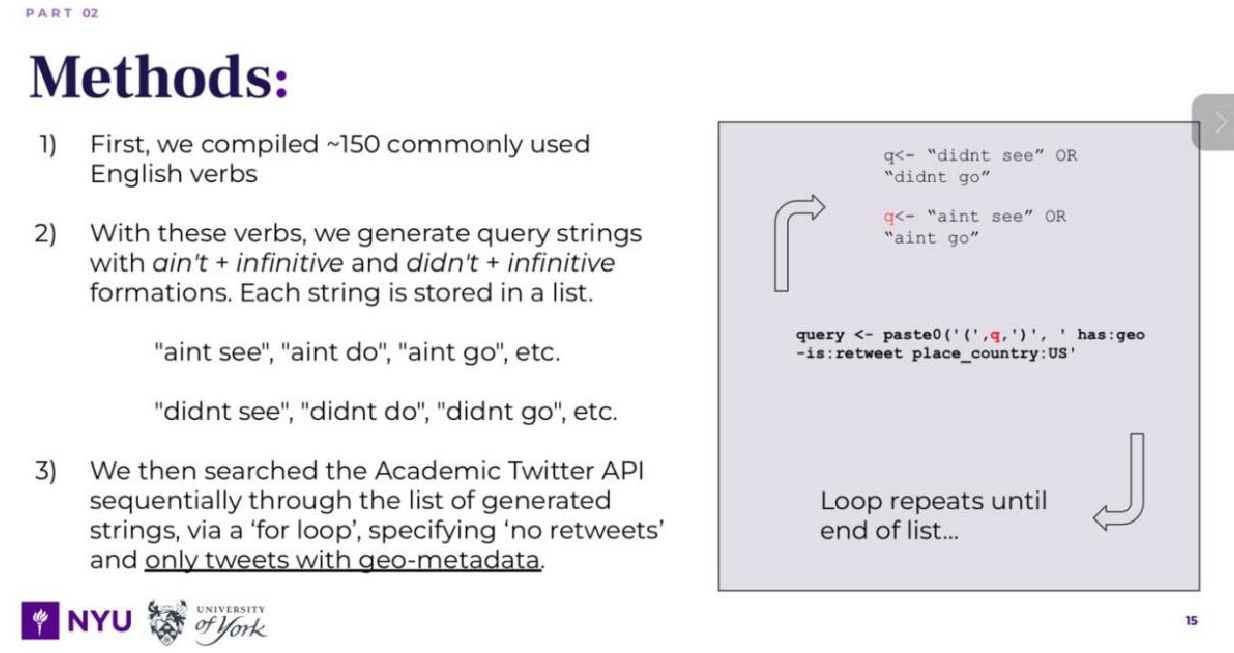
\includegraphics[width=\textwidth]{ExtractingNonStandardDatafromtheTwitterAPI-img001.png}
\caption{\citet{chapters/02-baxterEtAl}, slide 15; screenshot of loop for collecting tweets from the ACTW}
\label{fig:baxter:1}
\end{figure}

\figref{fig:baxter:1} is an image of the for loop used to collect data from the ACTW for \textit{ain’t-for-didn’t}. In the case of perfective \textit{done}, I search for \textit{done} + a list of approximately 150 commonly used verbs in their simple past and participle forms, while excluding the aforementioned “don’t count” \citep{Blake1997} cases. The resulting dataset extracted directly from ACTW was approximately 526,000 tweets.

I then examined the resulting data to check for FPs. I then arranged the tweets by “place name,” according to the metadata within each tweet. The place name is represented as “City, State” or “City, Territory” within the metadata, and represents the geographical location where the user was when they published the tweet. I first examine the output of a large city with between 5 and 10 thousand tweets (such as Charlotte) and then I document the “don’t count” and other cases therein which show high numbers of FPs. Some examples of constructions with a with high numbers of FPs are listed below. Queries are italicized, FPs are marked with a star*, and examples of perfective \textit{done} are marked with a check ✔.\pagebreak

\ea \textit{I’ve done drunk} %17
\ea [*]{I climbed onto a roof last night. Probably the \#1 unsafe thing I've done drunk}
\ex [✔]{I've done drunk my problems away before}
\z
\z

\ea  \textit{done done} %18
\ea [*]{\label{ex:baxter:18a}Done Donee done done done done done done.}
\ex [✔]{I done done a lot in my 21.9 years of my life}
\z
\z

\ea  \textit{done did} %19
\ea [*]{Done done done. Did I mention I was done?}
\ex  [✔]{And I done did everything but trust these hoes}
\z
\z

The most common FPs included \textit{be done, done done, have done}, contracted-copula \textit{done}, and \textit{done-}adverb constructions, including temporal adverbs such as \textit{just}, \textit{already}, and \textit{yesterday}. All of these can be used in perfective \textit{done} constructions (see \tabref{tab:baxter:1}); however, as mentioned above, due to the large number of FPs within the query results and/or the relative rarity of these cases among the data, they were eliminated.

After eliminating strings which were most likely to lead to FPs, 426,000 tweets of perfective \textit{done} remained. This set of tweets will hereafter be called the perfective \textit{done} dataset.

I calculate an index of perfective \textit{done} use in a similar way to the “straight” model outlined in \citep{RickfordEtAl1991}. As a result, it is necessary to find something to which perfective \textit{done} may be compared. As stated above, while perfective \textit{done} can be compared to the MAE perfect (\textit{has}/\textit{had}/\textit{have}), it is not identical. In addition, because it is not identical to the MAE perfect and because of the comparative robustness of the verbal TMA system in AAE, there is no single one-to-one yardstick to which perfective \textit{done} may be compared. In an attempt to solve this problem, I choose a calculation in which the \textit{perfective} \textit{done} \textit{dataset} is divided by all uses of \textit{done} taken from the same time period (2012--2015); this sample of 8.5 million tweets will hereafter be called the \textit{all done dataset}.

Both the \textit{perfective done dataset} and the \textit{all done dataset} are cleaned in several ways. First, all duplicate tweets are removed from each file to eliminate mass-duplicate tweets containing song lyrics and popular turns of phrase which may not be used in everyday speech. In addition, all utterances with three or more consecutive instances of \textit{done} are removed to eliminate utterances like the one in Example \REF{ex:baxter:18a}, which are not examples of perfective \textit{done}. Each dataset is then reduced to one tweet per user. This helps to eliminate the misrepresentation of tweets by individual users who tweet more heavily than others. I choose this method rather than the usual method of gathering proportions for each individual because this study frames perfective \textit{done} use in terms of how many twitter users in each location use perfective \textit{done}, rather than how many times each user uses perfective \textit{done,} or what proportion of use each user produces. Limiting tweets to one per user is a clear and straight-forward way to figure out how many twitter users produced the token within a given area.

Once each dataset is reduced to one-per-author, I extract the latitude, longitude, place name, and user id, and calculate a per-city count based on the number of tweets occurring within each location. For the \textit{perfective done dataset}, this count will be called the \textit{perfective done count}, and for the \textit{all done dataset}, this column will be called the \textit{all done count}.

I divide the perfective \textit{done} count by the \textit{all done} count, and the result is a series of indices reflective of the number of users who have used perfective \textit{done} with the selected 150 words in their tweets.

These indices (marked “newindex” on the right side of \figref{fig:baxter:2}) are mapped according to their geotag and assigned a color gradient, from dark blue for low indices and yellow for high indices. The resulting map is pictured below.

\begin{figure}
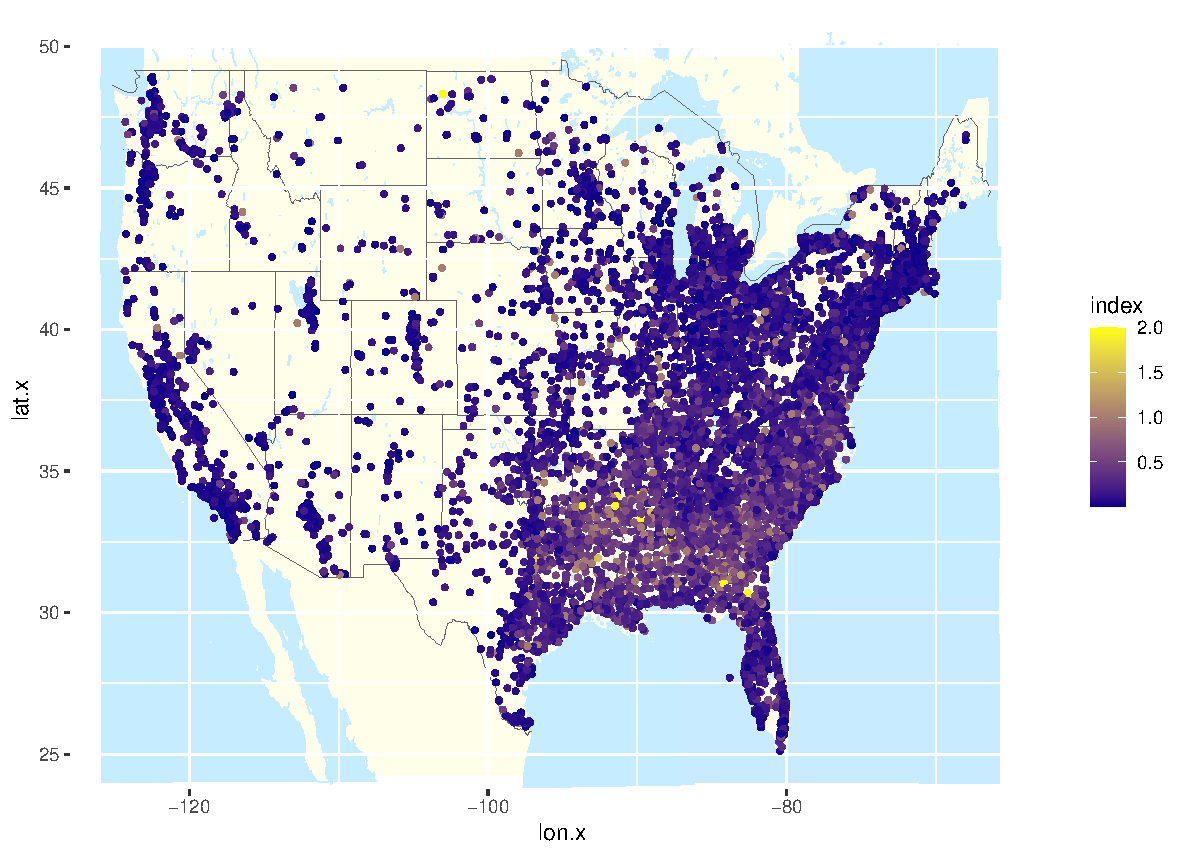
\includegraphics[width=\textwidth]{Figure 2_mod.pdf}
\caption{Front-End perfective \textit{done} map}
\label{fig:baxter:2}
\end{figure}

While the \textit{front-end} approach is effective for extracting perfective \textit{done} directly from the ACTW, it is not suitable for calculating indices of use for the following reasons:

\begin{itemize}
\item[I.]  The data extracted from the ACTW is not an exhaustive account of all tweets from that time period (\url{https://developer.twitter.com}). Rather, it is a collection of data from a given time period which, while still a good sample of Twitter use, may still include or exclude tweets from the \textit{all done dataset}, which was pulled from the ACTW separately, and is thus a separate sample. As a result, indices of certain towns and cities, especially those with a total of 30 user IDs or less, exhibit indices larger than 1. This should not be possible, since all uses of perfective \textit{done} should occur within the \textit{all done dataset}.

\item[II.]  In restricting the \textit{all done dataset} to one tweet per user ID, I did not account for the fact that the \textit{all done dataset} included \textit{perfective done dataset} tweets among its 8.5 million tweets.  If a user appearing in the \textit{all done dataset} used both perfective \textit{done} and verbal or other forms of \textit{done}, there is no way of knowing which tweet R would use to represent that user. As a result, the resulting 1.6 million tweets, restricted to one per user may not be representative of the \textit{unrestricted all done dataset}.

\item[III.]\sloppy  When comparing the \textit{perfective done dataset} to the \textit{all done dataset}, it quickly became apparent that the \textit{perfective done dataset} was missing a great many instances of perfective \textit{done} that still appeared in the \textit{all done dataset}.  This is because this method specifically searched for \textit{done} + {\textasciitilde}150 commonly used verbs. Those instances of \textit{done} were coded as perfective \textit{done}, while all instances of \textit{done} + other verbs were not coded and therefore not included in the \textit{perfective done dataset}, or coded as perfective \textit{done} within the \textit{all done dataset}.
\end{itemize}

As a result of these and other problems, I employ a different strategy to formulate the \textit{perfective done dataset} and calculate indices of perfective \textit{done} use.

\subsection{The back-end approach}
\label{sec:baxter:4.2}
Having already formulated the \textit{all done dataset} by extracting all uses of \textit{done} from the ACTW, I extract a new \textit{perfective done dataset} from the existing \textit{all done dataset}, rather than extracting the \textit{perfective done dataset} directly from the ACTW. This immediately remedies the issue of mismatching Twitter samples and by proxy eliminates the occurrence of indices greater than 1.

To do so, I create a list of all lemmas following \textit{done} among the 8.5 million tweets in the \textit{all done dataset}.

While reading all 8.5 million tweets is unfeasible within the given timespan of this study, there are only about 53,000 lemmas following \textit{done} in all 8.5 million tweets, including all alternate spellings of each word (e.g.: \textit{left}, \textit{leff}, \textit{lef}, etc.). I code all {\textasciitilde}53,000 lemmas manually and mark simple past forms, participle forms, and any alternate spellings therein with an \textit{x}. This takes roughly 18 hours, but is an incredibly important step in the creation of a database of alternate spellings of past-tense verbs, many of which may not have been predicted by simply guessing what ways users can and cannot spell things.

In addition to the “don’t count” \citep{Blake1997} cases above, I also do not mark \textit{un}{}-verbs, and other lemmas which can also be interpreted as adjectives because these are also likely to be FPs (e.g.: adjectives such as \textit{undone}, \textit{unloved}, etc.) I then code the resulting {\textasciitilde}3,900 marked tokens as perfective \textit{done} and all unmarked tokens as \textit{other}. I then extract all perfective \textit{done} coded tweets to create the new \textit{perfective done dataset}, and extract all \textit{other} coded tweets to a new dataset called the \textit{other dataset.}

 
\begin{figure}
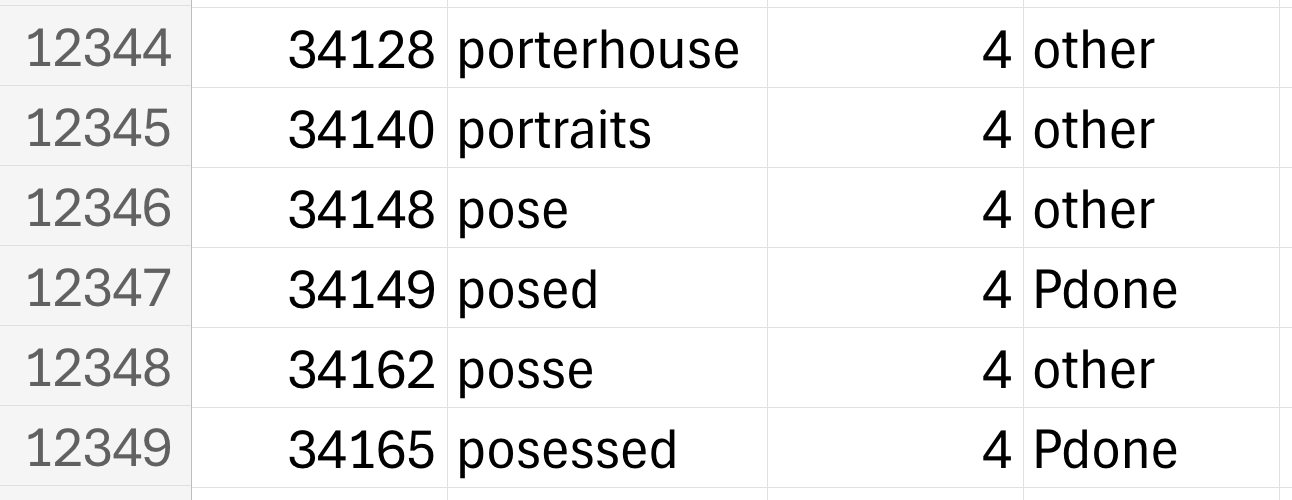
\includegraphics[width=0.7\textwidth]{figures/baxter/ExtractingNonStandardDatafromtheTwitterAPI-img003.png}
\caption{Sample image of perfective \textit{done} documentation}
\label{fig:baxter:3}
\end{figure}

Similarly to the \textit{front-end} method above, I restrict each file to one per user, and count the number of instances by city. I then calculate indices with the equation in example \REF{ex:baxter:19}.

\ea \label{ex:baxter:19}
\[ 
\text{perfective \textit{done} index} = \frac{\text{perfective \textit{done} count}}{\text{perfective \textit{done} count + other count}}
\]
\z

This new calculation of the perfective \textit{done} index addresses the user representation problem in the \textit{front-end} method, as speakers who use both perfective \textit{done} and other forms of \textit{done} now have both uses adequately represented in the denominator. Once the indices are calculated, I use geospatial mapping tools to map these indices across the contiguous United States as shown below in \sectref{sec:baxter:5}.

\section{Results and analysis} %5. /
\label{sec:baxter:5}

\begin{figure}
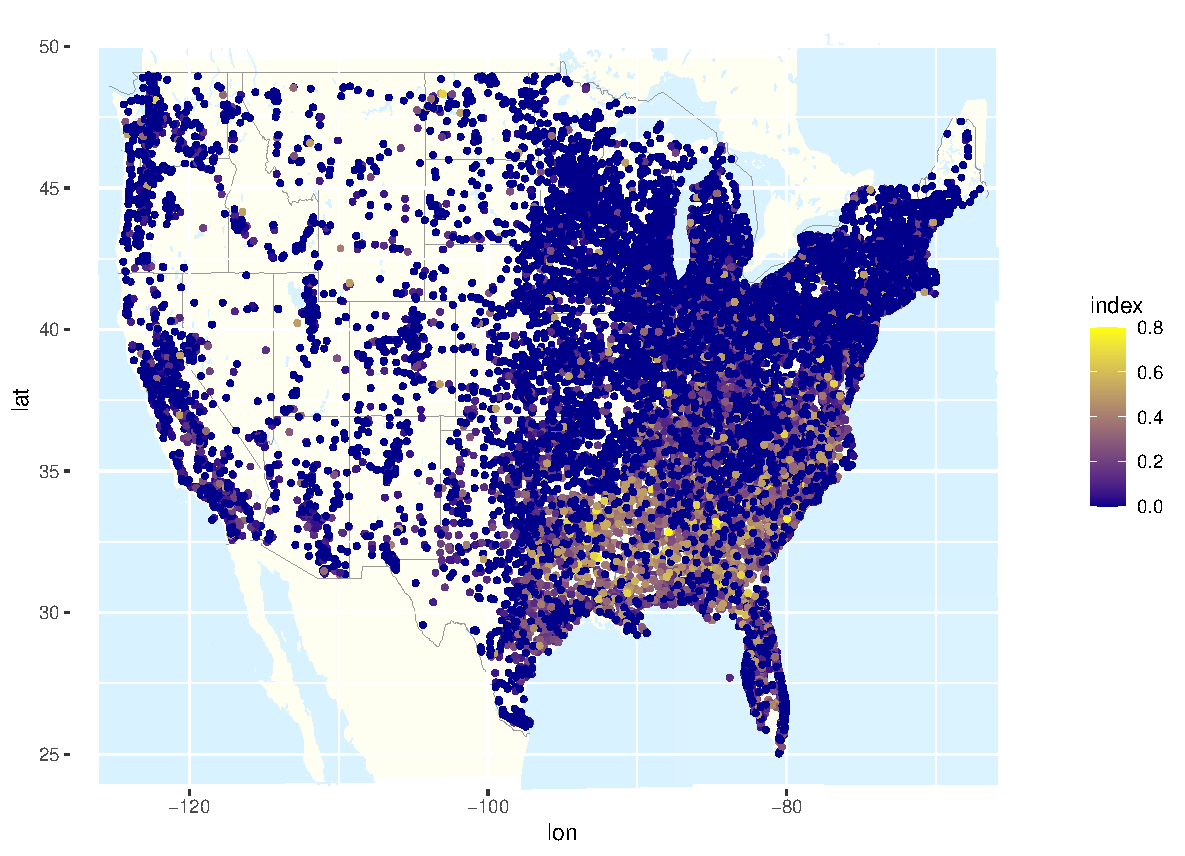
\includegraphics[width=\textwidth]{Figure 4_mod.pdf}
\caption{\label{fig:baxter:4} Perfective \textit{done} use in the contiguous United States}
\end{figure}

\figref{fig:baxter:4} is the map resulting from the \textit{back-end} approach mentioned above in \sectref{sec:baxter:4.2}. Bright (yellow) dots are representative of high perfective \textit{done} use, while dark (blue) dots are representative of low perfective \textit{done} use. A cluster of bright dots can be seen in the southeastern United States, which indicates higher indices of use in this region than in northern, or midwestern regions of the United States. Based on this, the data shows that perfective \textit{done} is more commonly used among Twitter users in the southeastern United States than in other regions.


To confirm these results, I cross-reference these perfective \textit{done} indices with BAA population rates in US Census Tracts in a selection of states representative of each region: Pennsylvania, New York, Illinois, Alabama, and Georgia. Each scatterplot is cropped down to their maximum perfective \textit{done} and BAA population indices. Where most states have some BAA populations that approach 100\%, thereby necessitating the need for the full 1.0 on the y-axis, the maximum indices on the x-axis vary widely. For example in \figref{fig:baxter:7} (Georgia), the maximum perfective \textit{done} index is approximately 0.7, whereas in \figref{fig:baxter:6} (New York), the maximum perfective \textit{done} index is 0.3. This is done for the sake of visibility in states where perfective \textit{done} indices are relatively low, so that the distribution of datapoints therein are still visible and interpretable.


\begin{figure}[p]
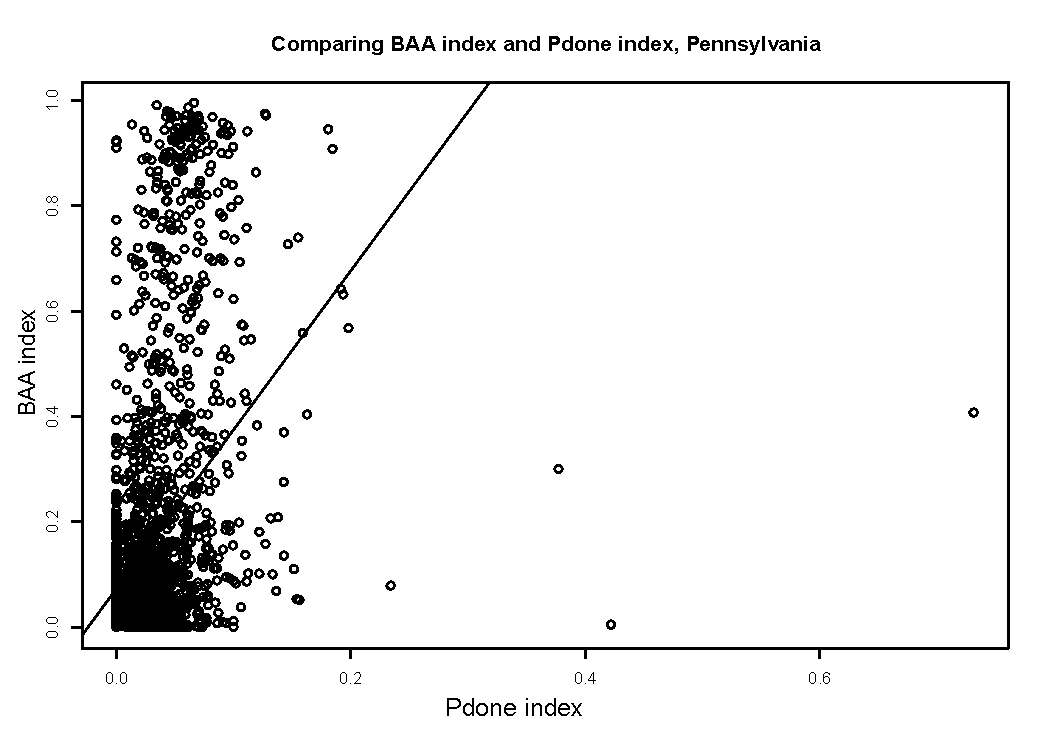
\includegraphics[height=.4\textheight]{PA_plot (2).pdf}
\caption{\label{fig:baxter:5} A comparison of the BAA index (vertical; BAA Population index)
and the perfective \textit{done} index (horizontal; Index of Perfective \textit{done} use
(Pennsylvania; PDONE MAX VALUE = approx. 0.8).}
\end{figure}


\figref{fig:baxter:5} is a scatter plot depicting a comparison of the BAA index: the percentage of BAA-identifying people living in a given area according to the US Census, to the perfective \textit{done} index: the percentage of users with perfective \textit{done} in their tweets. In Pennsylvania, among areas with high populations of BAA-identifying people, indices are relatively low, falling entirely below 0.2.

\begin{figure}[p]
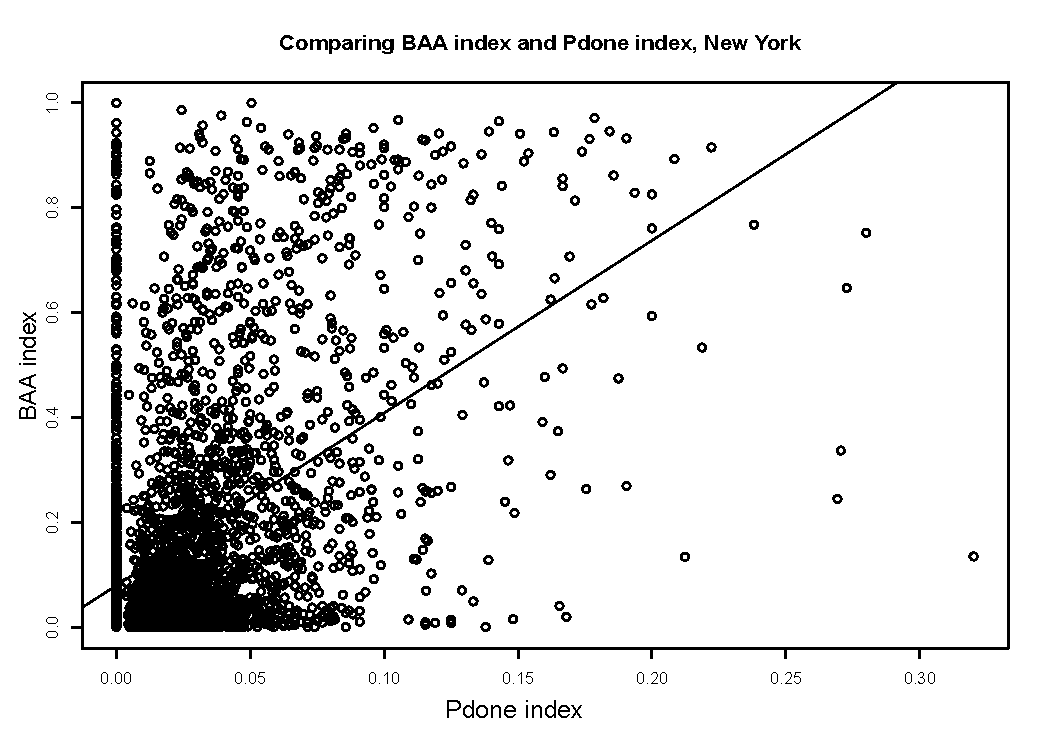
\includegraphics[height=.4\textheight]{NY_plot (3).pdf}
\caption{\label{fig:baxter:6} A comparison of the BAA index (vertical; BAA Population index)
and the perfective \textit{done} index (horizontal; Index of Perfective \textit{done} use. (New York; PDONE MAX VALUE = approx. 0.35)}
\end{figure}


\figref{fig:baxter:6} shows a similar trend to the one shown in \figref{fig:baxter:5}, with the maximum perfective \textit{done} index at just over 0.3 for any recorded locations in the state. Similarly to Pennsylvania, locations in New York with high populations of BAA-identifying people mostly show perfective \textit{done} indices of 0.2 or less, although very few are just above 0.2. Most notably, New York appears to show many locations with very low perfective \textit{done} indices. Many of these are flatly at the 0.00 mark.

\begin{figure}[p]
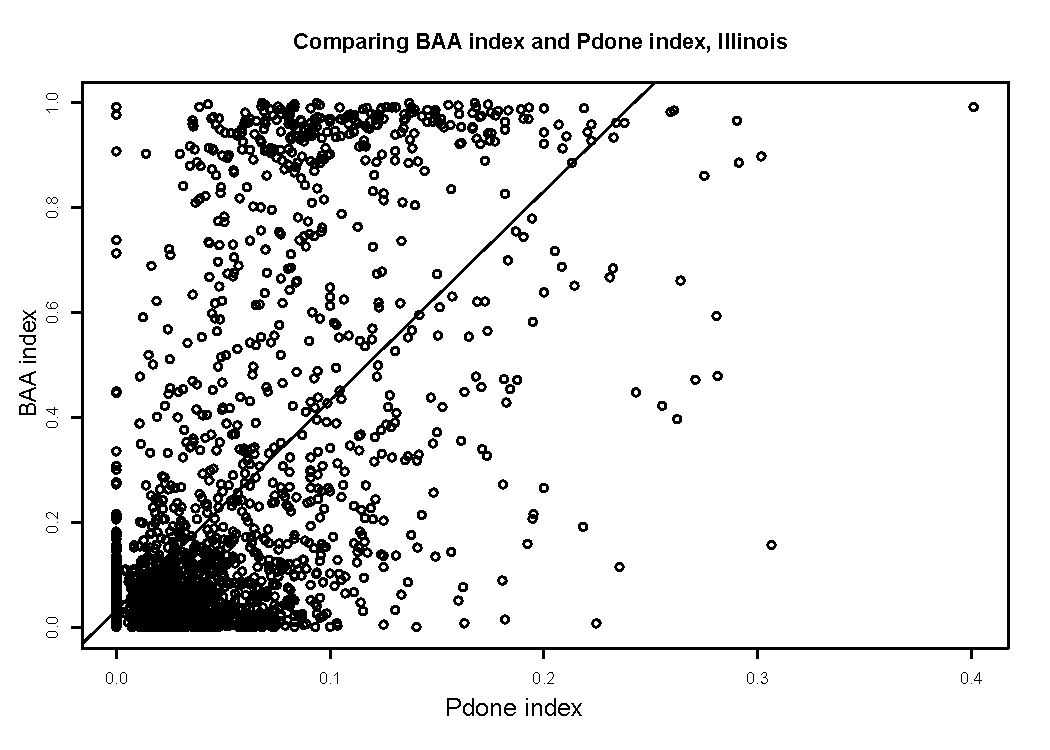
\includegraphics[height=.4\textheight]{IL_plot (2).pdf}
\caption{\label{fig:baxter:7} A comparison of the BAA index (vertical; BAA Population index) and the perfective \textit{done} index (horizontal; Index of perfective \textit{done} use. (Illinois; PDONE MAX = approx. 0.4)}
\end{figure}

\figref{fig:baxter:7} is a scatter plot from Illinois, which shows similar features to previous northern states. Similarly to New York, the maximum perfective \textit{done} index is 0.4. However, unlike New York, Illinois does not appear to show many locations with zero ratings. Rather, similarly to Pennsylvania, many locations with high BAA populations appear to be spread between the 0.0 and 0.2 mark, with several more between the 0.2--0.3 marks. While Illinois is a northern state, it is also located in the Midwest. The aforementioned divergence from northeastern states like New York whereby relatively few high-density BAA census tracts in Illinois show a 0.0 perfective \textit{done} index may be indicative of a broader trend in the Midwest. Conversely, it is also possible that New York is unique in its apparent rejection of perfective \textit{done} among Twitter users.


 
\begin{figure}[p]
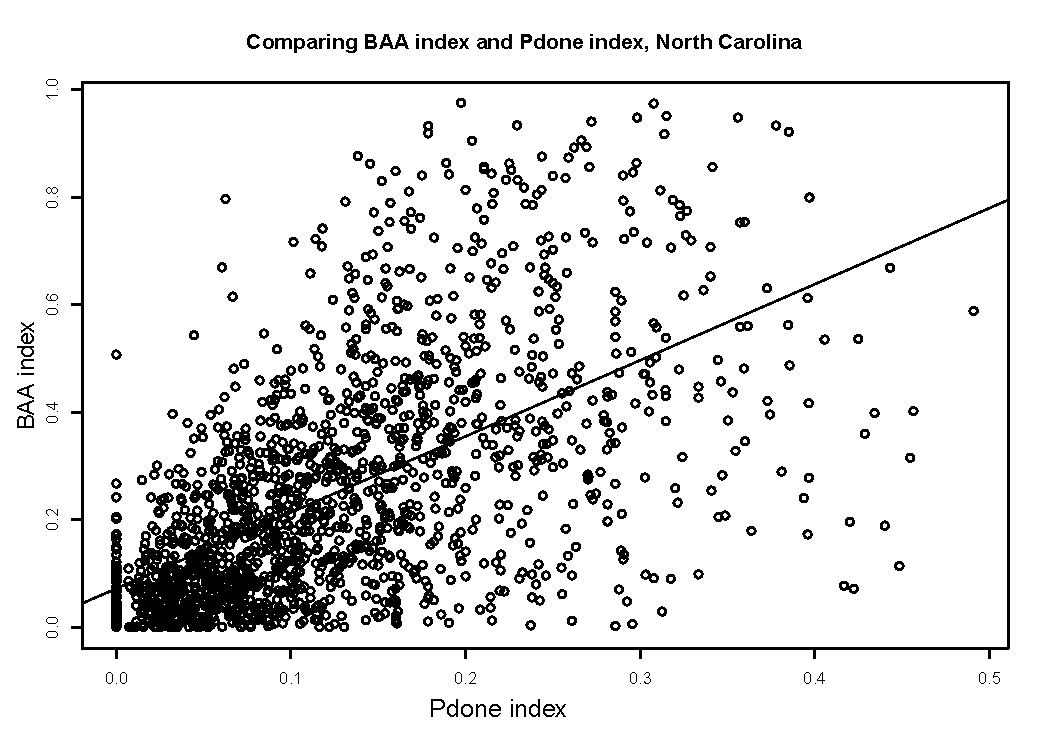
\includegraphics[height=.4\textheight]{NC_plot (2).pdf}
\caption{\label{fig:baxter:8} A comparison of the BAA index (vertical; BAA Population index) and the perfective \textit{done} index (horizontal; Index of Perfective \textit{done} use). (North Carolina, PDONE MAX VALUE = approx. 0.5)}
\end{figure}

\figref{ex:baxter:8} is a scatter plot of data taken from North Carolina. Where many locations with high BAA populations in Northern states appear to max out at between 0.2 or 0.3 perfective \textit{done} index, high BAA populations in North Carolina are mostly between 0.1 and 0.4, with none at the 0.00 mark.


 
\begin{figure}[p]
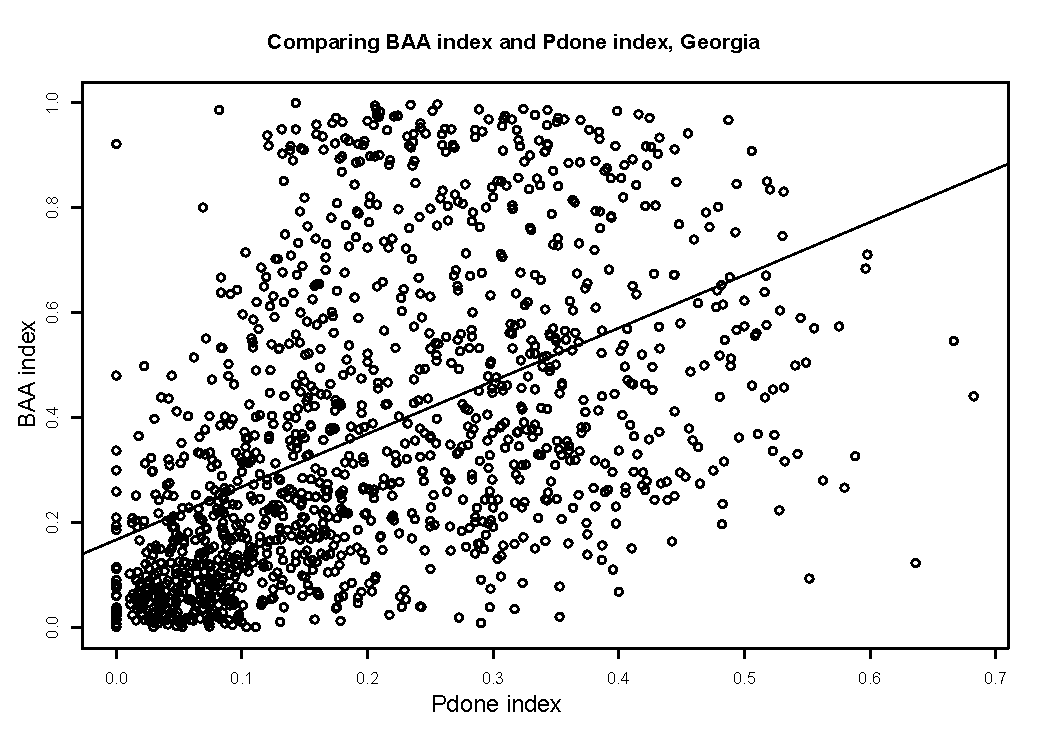
\includegraphics[height=.4\textheight]{GA_plot (2).pdf}
\caption{\label{fig:baxter:9} A comparison of the BAA index (vertical; BAA Population index) and the perfective \textit{done} index (horizontal; Index of perfective \textit{done} use). (Georgia; PDONE MAX VALUE = approx. 0.7)}
\end{figure}



\figref{fig:baxter:9} is a scatter plot of data taken from Georgia. Similarly to North Carolina, while there is one location with a high BAA population with a perfective \textit{done} index approaching 0.00, most others fall above 0.1, and show much wider distribution than Northern states, with indices ranging up to 0.5, which is higher than the maximum perfective \textit{done} index for all Northern states mentioned above except Pennsylvania, which has one outlier above 0.6.


\begin{figure}[p]
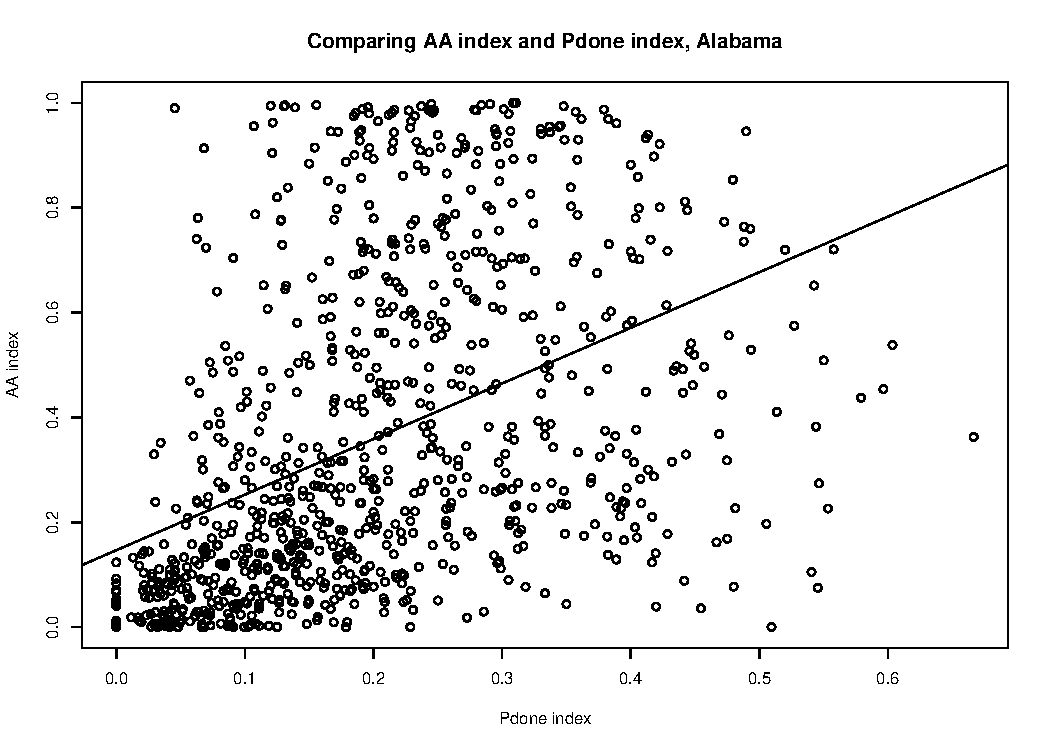
\includegraphics[height=.4\textheight]{AL_plot (2).pdf}
\caption{\label{fig:baxter:10}A comparison of the BAA index (vertical; BAA Population index) and the perfective \textit{done} index (horizontal; Index of Perfective \textit{done} use). (Alabama; PDONE MAX = approx. 0.7)}
\end{figure}


\figref{fig:baxter:10} is a scatter plot of data taken from Alabama. Similarly to Georgia and North Carolina, while there are two high BAA population locations which fall below the 0.1 mark, most others are diffused along a wider range from 0.1 to 0.5.

Scatterplots from northern states in the eastern and midwestern United States show a greater number of areas with high density populations of BAA people with lower indices of perfective \textit{done}. This indicates a lower rate of use, on average, of perfective \textit{done} among Twitter users in these regions. In contrast, scatterplots from Southeastern states show very few locations with high-density populations of BAA people who do not produce perfective \textit{done}. As indicated in Figures~\ref{fig:baxter:8}--\ref{fig:baxter:10}, maximum indices are higher, and the top left corner is empty or mostly empty, which indicates a lack of locations with high-density BAA populations and low perfective \textit{done} indices. Scatterplots of data taken from southeastern states also shows a wider distribution of perfective \textit{done} than northern cities.

These results confirm the hypothesis that regional differences in indices of perfective \textit{done} use will be reflected in the geospatial data, as shown in maps produced by both the \textit{front-end} and \textit{back-end} methods, as well as the scatterplots above. This also confirms the hypothesis that use of the perfect marker \textit{done} is more concentrated in the southeastern states than in northern states.

Additionally, variation in AAE can be mapped geospatially via the geolocation data included in tweets mined from the ACTW.

\section{Conclusion} %6. /
\label{sec:baxter:6}
This paper discusses the extraction of perfective \textit{done} and the geospatial mapping of indices of perfective \textit{done} use via the location data attached to each tweet. I discuss two methods of extracting perfective \textit{done} from the ACTW: a \textit{front-end} approach which aims to isolate uses of perfective \textit{done} by eliminating non-perfective uses of \textit{done} from the search prior to running the query, and a \textit{back-end} approach which first extracts a set of all uses of \textit{done} from 2012--2015 and aims to isolate uses of perfective \textit{done} afterwards. I conclude that while both methods are effective at extracting perfective \textit{done} from the ACTW, the \textit{back-end} approach is better suited to geospatial mapping.

The resulting map map shows a cluster of high indices of use in the southeastern United States, which indicates a higher concentration of perfective \textit{done} use among Twitter users therein. Indices of use of perfective \textit{done} were then cross-referenced with demographic data from the US Census. The resulting scatter plots showed that overall, Census tracts with high-density populations of BAA people in New York and Pennsylvania had much lower indices of perfective \textit{done} use than similar populations in Alabama, Georgia, and North Carolina. Not only does this challenge previous assumptions of a “uniform” AAE in urban centers across the United States, it indicates a likely correlation between region and perfective \textit{done} use, with northeastern states showing lower indices overall, and southeastern states showing higher indices overall. Illinois presents an interesting case wherein indices of perfective \textit{done} use in high-density BAA populations are slightly higher than northeastern states, but still lower than southeastern states. It may be that this middle-ground result is indicative of data taken from midwestern states~-- however, further study must be conducted regarding indices of use in other midwestern states.


Finally, I have shown that a language grouping approach is an appropriate method in the case of anonymized social media data which presents a variety of challenges in identifying and classifying the ethnicities of users. By using this approach and using demographic data taken from the US Census, I provide a broad yet comprehensive view of perfective \textit{done} usage rates in high-density BAA communities across the United States.


\section{Future research} %7. /
\label{sec:baxter:7}
In the future, I plan to add additional methods to this study to further legitimize the use of social media data and Census data to describe patterns in AAE on such a wide scale. I outline the next steps in this research below:

\begin{enumerate}
\item Investigate the new demographics of X (formerly Twitter), and conduct a deeper examination of how recent leadership, moderation, and other administrative changes have affected Black Twitter. Has the hostile environment outlined in \citet{Dwoskin2023} changed the way language is used among those who continue to use X?

\item Revisit the distribution of perfective \textit{done} in northern states and cities. Do BAA populations in New York, Pennsylvania, and other northeastern or mid-Atlantic states all show low indices of perfective \textit{done} use? Are there pockets of high use in any of these states?

\item Further examine perfective \textit{done} use in midwestern states.

\item Expand methodology to include sociolinguistic surveys and interviews, which are better suited toward topics around sociological grouping, such as racial and ethnic variation in AAE use among L1 speakers.

\item Investigate semantic and pragmatic variation in how perfective \textit{done} is used by the people who use it. While the categories in \citet{Comrie1976} fell short of encapsulating all potential uses of perfective \textit{done} in AAE, investigating distinctions between different types of perfective \textit{done} use is still valuable to our knowledge of how AAE works, how AAE is used, and by whom.

\item Investigate other parts of AAE speech to further deepen our understanding of language variation and change therein. 
\end{enumerate}

\section*{Abbreviations}

\begin{tabbing}
MMMMM \= Academic\kill
ADL   \> Academic Developer License  \\
ACTW  \> Academic Twitter API        \\
AAE   \> African American English    \\
BAA   \> Black/African American      \\
FPs   \> False Positives             \\
MAE   \> Mainstream American English \\
PDONE \> Perfective \textit{done}    \\
PERF  \> Perfect marker              
\end{tabbing}

\printbibliography[heading=subbibliography,notkeyword=this]
\end{document}
